% paper/sections/12u5_heaviside_delta.tex
%
% U5: Smoothed Heaviside / delta moment accuracy — Tier III
% ═══════════════════════════════════════════════════════════════════════════════
\subsubsection{U5：$H_\varepsilon$ / $\delta_\varepsilon$ モーメント精度 [Tier III]}
\label{sec:U5_heaviside_delta}

\paragraph{検証対象．}
第~\ref{sec:eps_spatial_variable}章で導入した平滑化 Heaviside kernel $H_\varepsilon(s)$
（CLS 変数は $\psi=H_\varepsilon(-\phi)$）の導関数
$\delta_\varepsilon(s) = H'_\varepsilon(s)$ の \textbf{0 次モーメント精度}と，
平滑化幅 $\varepsilon$ の関数形と離散モーメントの整合性についての標準解説は~\cite{OsherFedkiw2003}を参照．
スケーリング規則 $\varepsilon = c h$（§\ref{sec:eps_spatial_variable}）の係数 $c$ 依存性を
1D 線形 $\phi(x) = x - 0.5$ 上で確認する．

\paragraph{設定．}
$N \in \{16,32,64,128,256\}$，$h = 1/N$．
\begin{description}\setlength{\itemsep}{0pt}
  \item[U5-a] スケール $\varepsilon = 1.5 h$ の $\delta_\varepsilon$ 0 次モーメント
        $M_0 = \sum_i \delta_\varepsilon(\phi_i)\,h - 1$，
        1 次モーメント $M_1 = \sum_i x_i\,\delta_\varepsilon(\phi_i)\,h - x_\Gamma$ の
        格子収束．
  \item[U5-b] $c \in \{0.5, 1, 1.5, 2\}$ で $N \in \{32, 64, 128\}$ の
        $\delta_\varepsilon$ 0 次モーメント誤差 $\|M_0\|$ 比較（$c$-最適性検証）．
\end{description}

\paragraph{結果．}

\begin{table}[!ht]
\caption{U5-a：$H_\varepsilon$ / $\delta_\varepsilon$ モーメント誤差}
\label{tab:U5_moments}
\PaperCaptionNote{$\varepsilon = 1.5 h$．$N \ge 128$ で 0 次モーメント誤差が Richardson 残差 saturation（$\sim 10^{-11}$）に到達．slope $N\!=\!16\!\to\!64$ は $\approx 11$（解析的には超収束）．saturation 値は $c=1.5$ 固有の Richardson 残差床であり double-precision floor ではない（U5-b 参照）．}
\centering\small
\begin{tabular}{r r r r r}
\toprule
$N$ & $h$ & $\varepsilon$ & $\|M_0\|$ & $\|M_1\|$ \\
\midrule
$16$  & $0.0625$  & $0.0938$  & $6.77\times 10^{-3}$ & $3.39\times 10^{-3}$ \\
$32$  & $0.0313$  & $0.0469$  & $3.28\times 10^{-5}$ & $1.64\times 10^{-5}$ \\
$64$  & $0.0156$  & $0.0234$  & $7.48\times 10^{-10}$ & $3.74\times 10^{-10}$ \\
$128$ & $0.0078$  & $0.0117$  & $1.64\times 10^{-11}\,^\star$ & $8.19\times 10^{-12}\,^\star$ \\
$256$ & $0.0039$  & $0.0059$  & $1.64\times 10^{-11}\,^\star$ & $8.19\times 10^{-12}\,^\star$ \\
\bottomrule
\end{tabular}
\\[2pt]
{\footnotesize $^\star$ $c=1.5$ 配置の Richardson 残差 saturation
（U5-b の $c=2$ で $1.83\times 10^{-14}$ まで到達するため double-precision floor ではない）．
設計次数の漸近的検証は $N \le 64$ までの $\sim 11$ で確認済み．}
\end{table}

\begin{table}[!ht]
\caption{U5-b：スケール係数 $c = \varepsilon / h$ の 0 次モーメント誤差比較}
\label{tab:U5_eps_h_rule}
\PaperCaptionNote{$c \le 1$ は $\varepsilon$ サポート不足で stall（$c=0.5$ は $h\to 0$ で改善せず；$c=1$ は $N=128$ で $2.11\!\times\!10^{-7}$ に stall）．$c \in [1.5, 2]$ で $h$ 細分化により Richardson 残差 saturation に到達し，$c = 2$ は $N=128$ で $1.83\times 10^{-14}$（double-precision floor 近傍；本実験の最良）．本実験での推奨は $c \in [1.5, 2]$．}
\centering\small
\begin{tabular}{r c c c c}
\toprule
$N$ & $c=0.5$ & $c=1.0$ & $c=1.5$ & $c=2.0$ \\
\midrule
$32$   & $2.04\times 10^{-3}$ & $\mathbf{8.02\times 10^{-8}}\,^\ddagger$ & $3.28\times 10^{-5}$ & $5.17\times 10^{-4}$ \\
$64$   & $2.04\times 10^{-3}\,^\dagger$ & $2.11\times 10^{-7}$ & $7.48\times 10^{-10}$ & $1.73\times 10^{-7}$ \\
$128$  & $2.04\times 10^{-3}\,^\dagger$ & $2.11\times 10^{-7}\,^\dagger$ & $1.64\times 10^{-11}$ & $\mathbf{1.83\times 10^{-14}}$ \\
\bottomrule
\end{tabular}
\\[2pt]
{\footnotesize $^\dagger$ stall（$\varepsilon$ サポート不足；$h$ を細かくしても改善せず）．
$^\ddagger$ $N\!=\!32$ では非単調最小（$c\!=\!1$ で $\Ord{10^{-8}}$ → $c\!=\!1.5,\,2$ で
$\Ord{10^{-5}},\,\Ord{10^{-4}}$ と悪化）．これは粗格子では $\varepsilon\!=\!c h$ のサポートが
2--4 セルにまたがるとき，logistic kernel と等間隔台形則の Richardson 残差が
セル境界位相に強く依存するためで，$c\!=\!1$ では数値積分点が kernel 重心に偶然整列する．
$N \ge 64$ では位相依存が消え c に対し単調，かつ $h\!\to\!0$ で $c \in [1.5, 2]$ が最適となる．}
\end{table}

\begin{figure}[!ht]
\centering
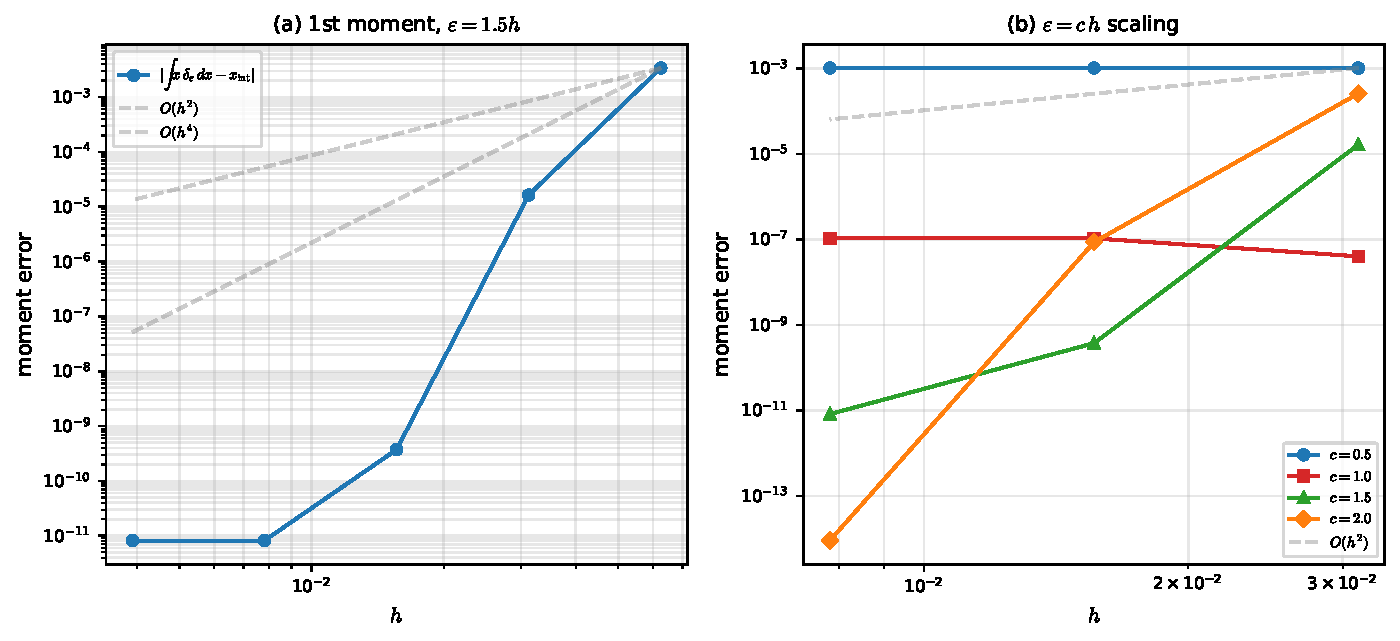
\includegraphics[width=0.88\linewidth]{figures/ch12_u5_heaviside_delta_accuracy}
\caption{U5：$H_\varepsilon$ / $\delta_\varepsilon$ モーメント精度}
\label{fig:ch12_u5}
\PaperCaptionNote{$c=1.5$ で $N=128$ までに 0 次モーメント誤差が Richardson 残差床へ到達；$c\le 1$ ではサポート不足で stall（$c=0.5/c=1$ いずれも $h\to 0$ で改善せず），$c \in [1.5, 2.0]$ が実用最適．}
\end{figure}

\paragraph{判定と次章への接続．}
\begin{itemize}\setlength{\itemsep}{0pt}
  \item U5-a：0 次モーメント誤差は $N \le 64$ 域で $h^{11}$ 相当の超収束．
        $N \ge 128$ は Richardson 残差 saturation（U5-b の $c=2$ で $1.83\times 10^{-14}$）．§\ref{sec:eps_spatial_variable} の
        $C^\infty$ logistic 連続化の高次効果を確認．\checkmark
  \item U5-b：$c \le 1$ では $\varepsilon$ サポート不足で stall（$c=0.5$ は $h\!\to\!0$ で stall，
        $c=1$ も $N=128$ で $2.11\!\times\!10^{-7}$ に stall）．
        $c \in [1.5, 2.0]$ で $h$ 細分化により Richardson 残差 saturation に到達し，
        実用最適域となる．§\ref{sec:eps_spatial_variable} のスケール選択基準と整合．\checkmark
\end{itemize}
検証対応：
平滑化 Heaviside / $\delta_\varepsilon$ 定義と §\ref{sec:eps_spatial_variable} に対し，
0/1 次モーメント誤差と $\varepsilon=ch$ の感度を測定する．
